\section*{Results}

This section deals with the presentation and discussion of results.
The collected data are related to the obtained reward from the artificial neural network of the project.
With these data is possible to see what is the learning degree of the agent in the environment because the gained reward is intrinsically attached to the performance of the agent on the environment that it must go.
All the training environments were arranged by ROBOTIS, however, some alterations were done on the source code of the Gazebo simulation in order for the simulated mobile robot to use the reward system defined on this paper.

A mobile robot with a DDPG network was trained in order to make the experiments in the environments presented on Fig. \ref{fig:environments}, where the goal of the mobile robot is to get to the target.
For the first test was used the first environment that shows, in Fig. \ref{fig:amb1target}, a sequence of frames of the robot and the target. We can observe how the robot start in an initial position distant from the target, navigating in order to reach the target.

\begin{figure}[H]
\centerline{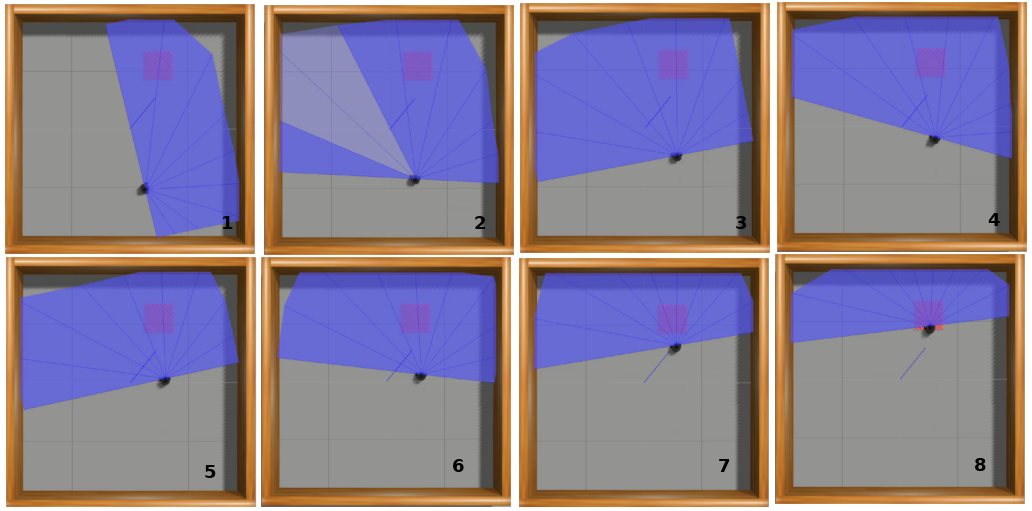
\includegraphics[width=\columnwidth]{images/amb1target.png}}
\caption{Images sequence in the first environment.}
\label{fig:amb1target}
\end{figure}

The training results of the reward function of the first environment are shown in Fig. \ref{fig:stage_1}.
On the first episodes can be noticed a negative reward, this happens because the algorithm started and it was still learning. 
This reward by episode means that the robot is trying to maximize the reward to complete the task. 
It is observed in the episode 400 a fall. 
This is a probable correction on some maximized parameters of the network and it resulted in a low reward.
Results like this means that the network has a continuous learning trying to correct itself. 

\begin{figure}[H]
\centerline{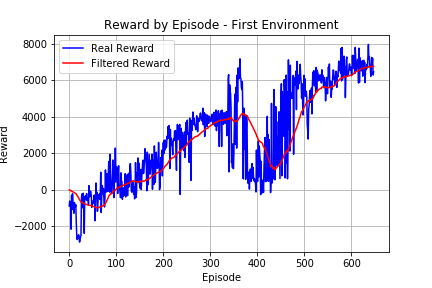
\includegraphics[width=10cm]{images/stage_1.png}}
\caption{Rewards of the first environment.}
\label{fig:stage_1}
\end{figure}

In Fig. \ref{fig:stage_1} the $x$ axis represents the past episodes on the simulation, an episode is defined when the mobile robot arrives to the target in the map or collides with some obstacle. 
The $y$ axis in Fig. \ref{fig:stage_1} represents the total value of the reward that the robot received on the episode.
The reward, with the blue color, has a great variance, it was decided to use a moving average filter for better visualization of the results.

After the mobile robot has been trained on the first environment, the experiment was done in the second environment and tested. It is shown in Fig. \ref{fig:amb2target} a sequence of the actions made by the TurtleBot from an initial position until it could arrive to the target after the training episodes.

\begin{figure}[H]
\centerline{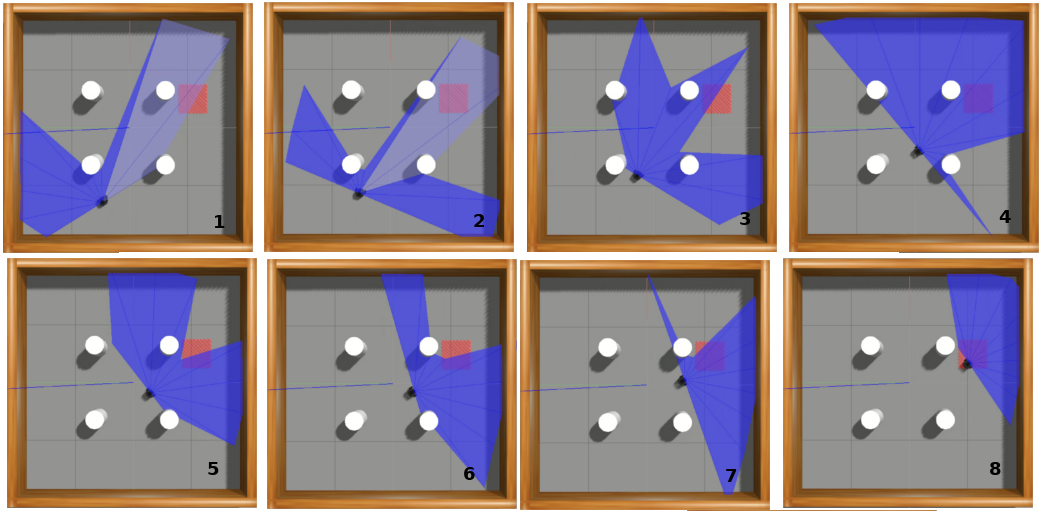
\includegraphics[width=\columnwidth]{images/amb2target.png}}
\caption{Images sequence in the second environment.}
\label{fig:amb2target}
\end{figure}

The reward function results of the training process for the second environment are shown in Fig. \ref{fig:stage_2}.
Comparing this results with the last environment, we can observe that it needed more episodes so the robot could present good results.
It is noticed that with a more complex environment, exists the possibility that an agent could take a longer time to get a good performance.

\begin{figure}[H]
\centerline{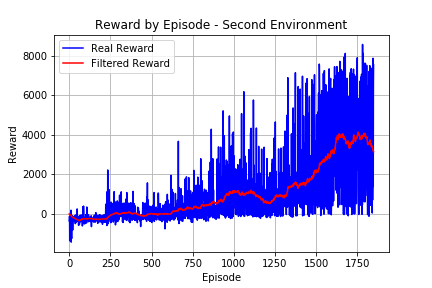
\includegraphics[width=10cm]{images/stage_2.png}}
\caption{Rewards of the second environment.}
\label{fig:stage_2}
\end{figure}

For the final test and the sequence of the actions made by the TurtleBot to arrive to the target after the training process it was used the third environment.  A sequence of the actions made by the TurtleBot to arrive to the target after the training episodes are shown in Fig. \ref{fig:amb3target}.

\begin{figure}[H]
\centerline{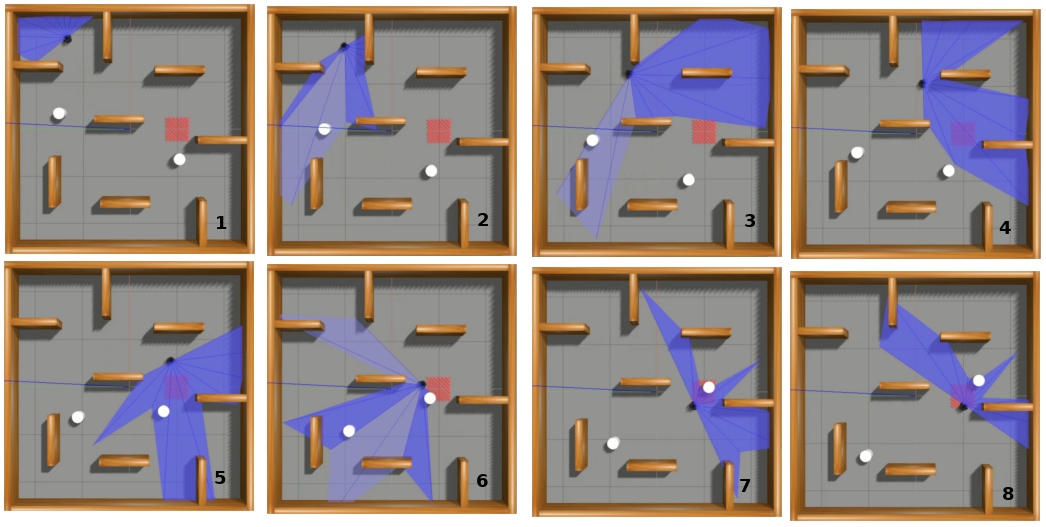
\includegraphics[width=\columnwidth]{images/amb3target.png}}
\caption{Images sequence in the third environment.}
\label{fig:amb3target}
\end{figure}

The results of the reward function of the last training environment is shown in Fig. \ref{fig:stage_4}.
On this environment, due to the high complexity, it was necessary a higher number of training episodes.
If compared the reward function with the previous Fig. \ref{fig:stage_1} and Fig. \ref{fig:stage_2}, it is possible to notice an average reward bellow two thousand.
This happens because to reach the target, which has the highest reward possible on comparison with the others, it is necessary that the agent could execute actions that do not generate too many points, however, that still makes it to arrive to the target.
Nevertheless, it was noticed by simulating the trained robot some actions that caused it to collide.
Many of these collisions were due to the moving dynamic obstacle close to the target.
This resulted in the agent making the decision of that mobile robot would collide or would try to avoid the obstacle.
The occurred behavior may have been caused because of the system created.
In order to resolve these actions, probably, it would be necessary to create a reward system that could bypass the error of the network.

\begin{figure}[H]
\centerline{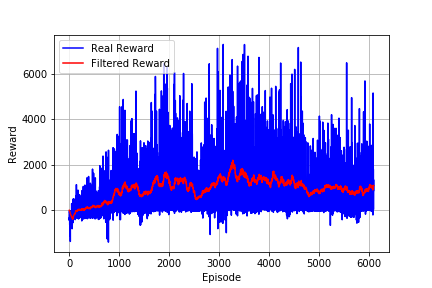
\includegraphics[width=10cm]{images/stage_4.png}}
\caption{Rewards of the third environment.}
\label{fig:stage_4}
\end{figure}

% Continua

After the training and validation of each simulation environment, it was created two more environments for the testing of the DDPG network in the real world.
The first real environment is shown in Fig. \ref{fig:real_envs} (a) and resembles the first simulation with no obstacles. The second environment is shown in Fig. \ref{fig:real_envs} (b) and it presents a complex environment similar to the second and third used on simulation with the exception of not having moving obstacles.

\begin{figure}[H]
\centerline{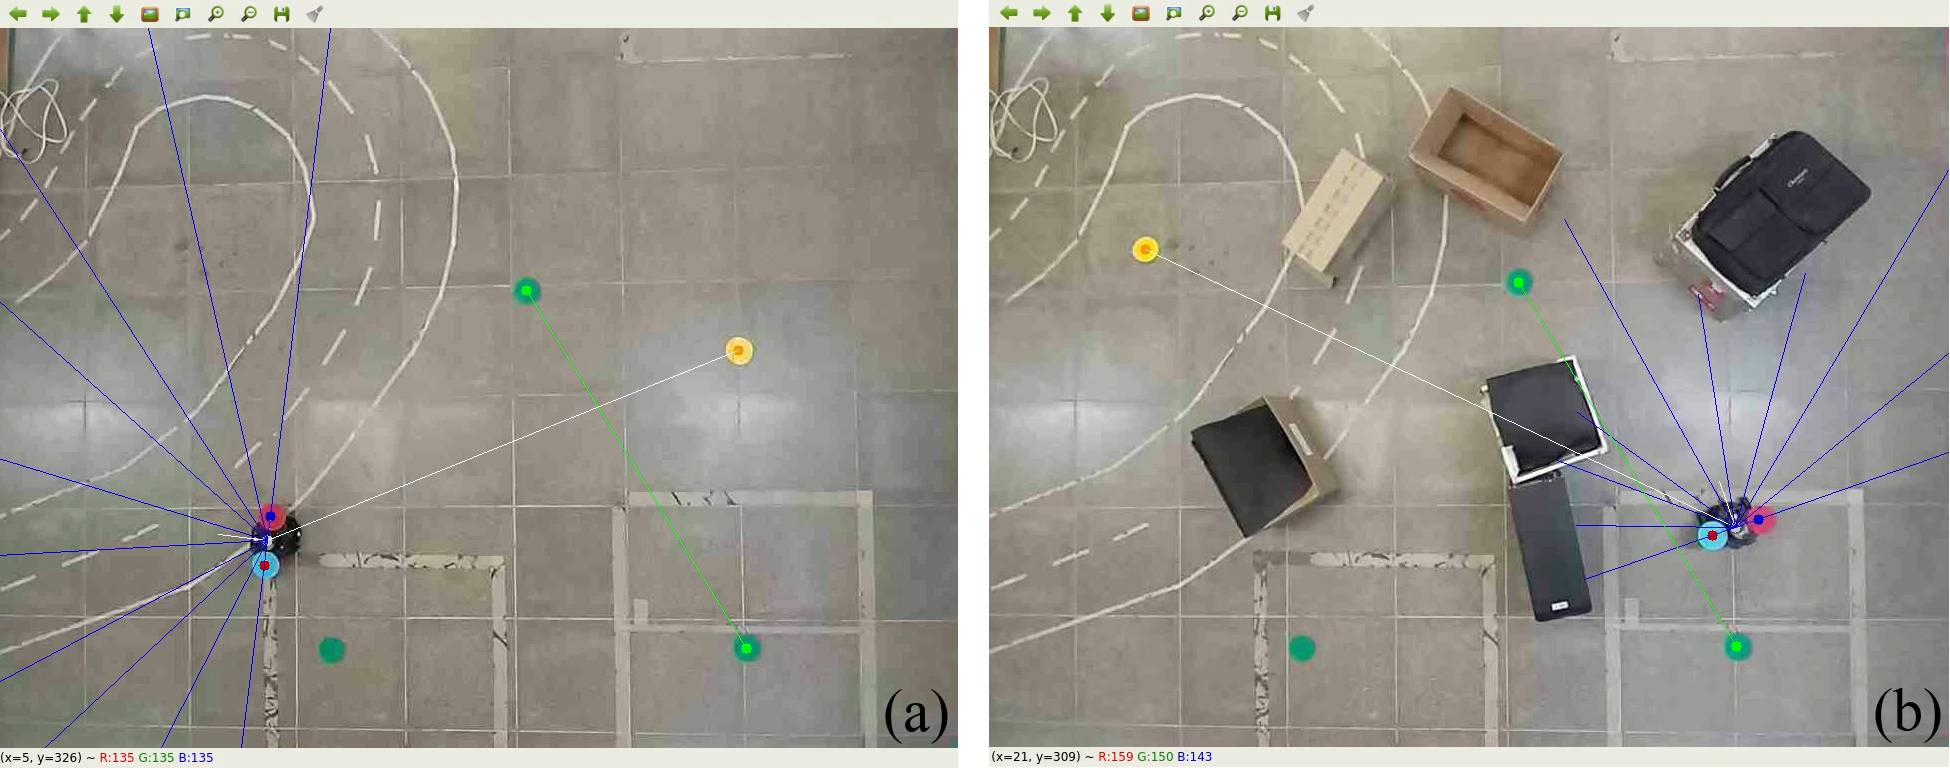
\includegraphics[width=12cm]{images/real_envs.png}}
\caption{Environments created for the DDPG test on the real world. First environment (a) and second environment(b).}
\label{fig:real_envs}
\end{figure}

With the target defined on the first real environment, it was executed the DDPG network on the Turtlebot3.
In the graph, shown in Fig. \ref{fig:env1_graph}, is possible to see the trajectory made by the network to arrive to the target.
In the Fig. \ref{fig:frames_env1} is shown by frames the trajectory made my the robot to complete the task.

\begin{figure}[H]
\centerline{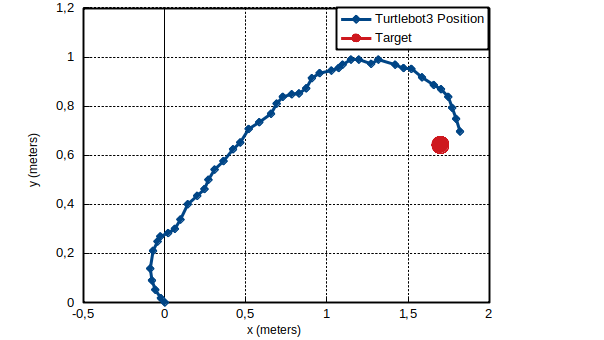
\includegraphics[width=12cm]{images/env1_graph.png}}
\caption{Trajectory of the Turtlebot3 in the first real environment}
\label{fig:env1_graph}
\end{figure}

\begin{figure}[H]
\centerline{\includegraphics[width=\columnwidth]{images/frames_env1.png}}
\caption{Images sequence of the Turtlebot3 in the first real environment}
\label{fig:frames_env1}
\end{figure}

For final test of the network, it was used the second real environment. In the graph, shown in Fig. \ref{fig:env2_graph}, even with obstacle the network was capable to arrive to the target. In the Fig. \ref{fig:frames_env2} is shown by frames the trajectory made my the robot to complete the task. %So, with these results applied on real world environment we can see how effective can be a DDPG network trained in simulation environment
The robot was able to accomplish both task given in the real world environments.
This shows how effective can be the DDPG networks, trained in a simulation environment, in completing complex tasks on physical environment.

\begin{figure}[H]
\centerline{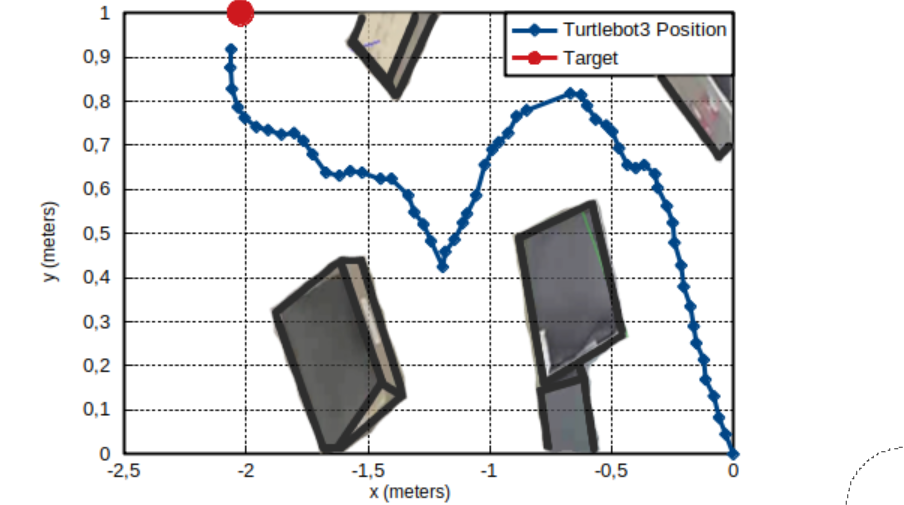
\includegraphics[width=12cm]{images/env2_graph.png}}
\caption{Trajectory of the Turtlebot3 in the second real environment}
\label{fig:env2_graph}
\end{figure}

\begin{figure}[H]
\centerline{\includegraphics[width=\columnwidth]{images/frames_env2.png}}
\caption{Images sequence of the Turtlebot3 in the second real environment}
\label{fig:frames_env2}
\end{figure}